\documentclass[11pt,a4paper]{article}
\usepackage[T1]{fontenc}
\usepackage[utf8]{inputenc}
\usepackage{lmodern}
\usepackage[margin=25mm]{geometry}
\usepackage{microtype,amsmath,amssymb,booktabs,tabularx,array}
\usepackage{tikz}
\usetikzlibrary{arrows.meta,positioning,fit,backgrounds}
\usepackage[section]{placeins}
\usepackage{graphicx}
\usepackage[font=small,labelfont=bf]{caption}
\raggedbottom
\clubpenalty=10000
\widowpenalty=10000
\displaywidowpenalty=10000
\renewcommand{\topfraction}{0.9}
\renewcommand{\bottomfraction}{0.8}
\renewcommand{\textfraction}{0.08}
\renewcommand{\floatpagefraction}{0.8}
\setlength{\floatsep}{12pt}
\setlength{\textfloatsep}{14pt}
\setlength{\intextsep}{12pt}
\makeatletter
\setlength{\@fptop}{0pt}
\setlength{\@fpsep}{16pt}
\makeatother
\definecolor{studyblue}{HTML}{0072B2}
\definecolor{studyorange}{HTML}{D55E00}
\definecolor{studygreen}{HTML}{009E73}
\tikzset{box/.style={draw=studyblue!75,fill=studyblue!5,rounded corners=2pt,align=center,inner sep=7pt,font=\small},arrow/.style={-{Stealth[length=2mm]},thick,draw=black!65},note/.style={font=\small,align=center}}
\usepackage[numbers,sort&compress]{natbib}
\usepackage[colorlinks=true,linkcolor=blue,citecolor=blue,urlcolor=blue]{hyperref}
\setlength{\parskip}{3pt}
\setlength{\parindent}{1em}
\newcolumntype{Y}{>{\raggedright\arraybackslash}X}
\title{Evaluating Source Layout and Access to Preservation Checks\\for Agent-Driven Feature Extension\\in Next.js SaaS Starter Kits}
\author{Do Hoang Trieu\\Vietnamese--German University}
\date{}
\begin{document}
\maketitle
\begin{abstract}
When a coding agent adds a feature to an existing application, its patch must also preserve behavior users already rely on. We propose an exploratory $2\times2$ experiment that varies source layout and access to runnable preservation checks. We will run the same three account tasks in Next.js SaaS Starter and Makerkit Lite across 48 planned agent sessions. We will score the requested feature and specified existing behavior separately and estimate how each intervention changes the share of patches that pass both and meet the study rules. To check the scoring before collecting agent data, we ran 72 evaluations on baselines and prepared patches. The task-specific checks detected all 24 deliberate regressions.
\end{abstract}

\section{Introduction}
Adding a feature to an existing application means changing one behavior while keeping others working. Consider an agent asked to add a confirmation dialog to a sign-out button. The dialog should appear and accept the user's choice. When the user confirms, the existing sign-out operation should still end the session. We call checks of the requested behavior \emph{acceptance checks} and checks of specified existing behavior \emph{preservation checks}.

Two changes to the agent's workspace could affect whether its patch passes both. Grouping related files may help the agent find the code it needs. Giving the agent runnable preservation checks may help it catch regressions before submission, at the cost of time spent running the checks. SWE-bench and SWE-Bench Pro measure agents' ability to change repositories~\cite{jimenez2024swebench,deng2025swepro}. Studies of agent instructions, repository precedents, and structural requirements show that how a task and codebase are presented can affect agent performance or implementation choices~\cite{gloaguen2026agents,zhu2026precedent,dente2026constraint}.

Prior work measures whether features and existing behavior continue to work, examines follow-on agent edits, or varies the verification tools agents can use~\cite{wang2026featurearc,feng2026featureloop,chen2026featbench,patel2026codethread,mehta2026verification}. Related experiments vary code cleanliness while matching application behavior~\cite{trivedi2026cleanliness}. Our study asks how source layout and access to preservation checks affect the same feature-extension tasks when we vary both in the same experiment.

We will run the same three account tasks in Next.js SaaS Starter and Makerkit Lite~\cite{nextjsSaasStarter,makerkitLite}. Within each kit, the $2\times2$ design compares the original and reorganized source layouts at both levels of check access. The design lets us estimate each change while holding the other fixed and describe whether the two changes interact. A patch counts as a \emph{joint success} if it passes both sets of behavioral checks and meets the common study requirements.

\section{Research questions}
The questions concern the three matched account tasks in the two selected kits.
\begin{samepage}
\begin{enumerate}
\item[RQ1.] How often do patches pass the acceptance and preservation checks in each condition, and what fails when they fall short?
\item[RQ2.] How much does reorganizing source files change the joint success rate across the selected tasks, within each kit and on average across kits?
\item[RQ3.] How much does supplying extra preservation checks change the joint success rate across the selected tasks, within each kit and on average across kits?
\end{enumerate}
\end{samepage}

Moving related modules may help agents find relevant code, and the effect may differ by kit. We expect the extra checks to increase joint success by helping agents detect regressions before submission. We will describe check use and time spent checking to help interpret the estimated effect of access to the package.

\section{Background and related work}\label{sec:related-work}
\subsection{Repository organization and code navigation}
Parnas links module decomposition to the changes that a module localizes~\cite{parnas1972modules}. Zhu et al. show that repository precedents can influence agent implementation choices. Their local-versus-sibling comparison also varies task relatedness~\cite{zhu2026precedent}. Trivedi and Schmitt vary naming, factoring, and complexity in matched repositories. They report lower token use and fewer file revisitations on cleaner code, with little change in the fraction of hidden tests passed~\cite{trivedi2026cleanliness}. We vary the locations of selected files and update their imports while holding tested application behavior fixed.

Studies of coding-agent context files show why instruction exposure warrants control alongside file placement~\cite{khatri2026context,gloaguen2026agents}. Information position also affects retrieval in long contexts~\cite{liu2024lost}. We examine navigation directly through the files agents read and revisit.

\subsection{Verification feedback during an agent session}
Mehta varies verification tools during web-application construction, including access to a tool for writing and running behavioral tests~\cite{mehta2026verification}. TDAD uses code--test dependencies to direct regression checks~\cite{alonso2026tdad}. FeatureLoop and Reflexion examine feedback across changes or trials~\cite{feng2026featureloop,shinn2023reflexion}. We start each session from the task baseline and let agents write their own tests in every condition. The intervention supplies checks that are ready to run against specified existing behavior.

\subsection{Evaluating the feature and existing behavior}
FeatBench uses fail-to-pass tests for new behavior and pass-to-pass tests for existing behavior~\cite{chen2026featbench}. FeatureArc applies that distinction over successive extensions in a persistent session~\cite{wang2026featurearc}. We apply it to individual patches from fresh sessions and record structural compliance separately, following the distinction between behavior and compliance in Constraint Decay~\cite{dente2026constraint}. Studies of downstream maintainability examine a separate question about how later work fares on generated code~\cite{patel2026codethread,borg2026echoes}.

\section{Experimental design}\label{sec:method}
Each of the \textbf{48 planned agent sessions} is one attempt at one task in a fresh workspace. The design crosses two kits, three matched tasks, and four workspace conditions, with two sessions per combination. For example, we will run the sign-out task in one starter kit twice under each of the four conditions, for eight agent sessions.
\subsection{What the agent will implement}
The three constructed tasks specify the same user-facing change and preservation requirements in both kits. Table~\ref{tab:tasks} summarizes the task cards. The final evaluator will exercise equivalent scenarios through each kit's own interfaces.

\begin{table}[ht]
\small
\renewcommand{\arraystretch}{1.16}
\caption{Matched account tasks and requirements}
\label{tab:tasks}
\begin{tabularx}{\linewidth}{@{}>{\raggedright\arraybackslash}p{0.25\linewidth}YY@{}}
\toprule
Proposed change & Required existing behavior & Acceptance check\\
\midrule
Display-name normalization & Opening settings displays legacy names exactly as stored. & Saving trims outer whitespace, retains internal spacing, and persists across reload.\\
Sign-out confirmation & After confirmed sign-out, a fresh request to a protected page requires sign-in. & The native dialog supports confirmation and cancellation, including keyboard activation. Cancel retains the session.\\
Sign-in password visibility & The sign-in field starts masked. Sign-up masking and autocomplete are preserved. & The Show/Hide button toggles masking via keyboard, retains the typed value, and leaves the form unsubmitted.\\
\bottomrule
\end{tabularx}
\end{table}

We derive preservation requirements from agreed specifications, existing tests, or confirmed domain rules. Agents receive the full requirements. The final evaluator can use withheld inputs. Before collection, we will check task descriptions for ambiguities and confirm that the workspaces and available repository history give agents no access to the prepared solutions~\cite{xia2024agentless}.

\subsection{What changes between conditions}
Both kits use the four conditions in Figure~\ref{fig:factorial}. Within a column, the agent receives the same checks and we compare two layouts. Within a row, the layout stays fixed and we compare two levels of check access.

\begin{figure}[htbp]
\centering
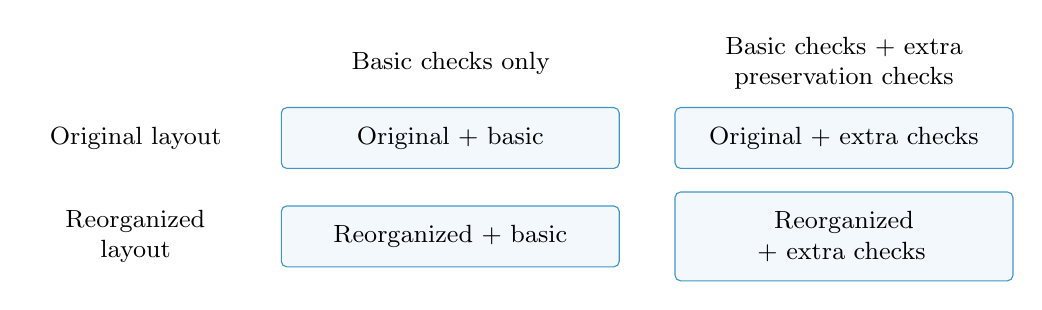
\begin{tikzpicture}
\node[note,text width=4cm] at (4,0.95) {Basic checks only};
\node[note,text width=4cm] at (9,0.95) {Basic checks + extra\\preservation checks};
\node[note,text width=2.5cm] at (0,0) {Original layout};
\node[note,text width=2.5cm] at (0,-1.25) {Reorganized layout};
\node[box,text width=3.8cm] at (4,0) {Original + basic};
\node[box,text width=3.8cm] at (9,0) {Original + extra checks};
\node[box,text width=3.8cm] at (4,-1.25) {Reorganized + basic};
\node[box,text width=3.8cm] at (9,-1.25) {Reorganized + extra checks};
\end{tikzpicture}
\caption{Experimental conditions}
\label{fig:factorial}
\end{figure}


\noindent\textbf{Basic checks (all four conditions).}
These checks cover TypeScript and the core account flows shared by the three tasks. They verify that the code passes TypeScript type checking, the registration page responds successfully, unauthenticated requests to a protected page redirect to sign-in, and a test account can sign in and access that page. Agents in $V=0$ receive only these checks.

\noindent\textbf{Supplied preservation checks (the two $V=1$ conditions).}
Agents also receive one runnable check for existing behavior that their assigned task could break. The check depends on the task:
\begin{itemize}
\item \textbf{Display-name normalization.} Opening account settings shows a legacy name exactly as stored, including leading and trailing whitespace.
\item \textbf{Sign-out confirmation.} After the user confirms sign-out, a fresh request to a protected page in the same browser session requires sign-in again.
\item \textbf{Sign-in password visibility.} When the sign-in page first opens, the password field is masked.
\end{itemize}

All agents receive the same task requirements and may write and run their own checks. The final evaluator scores acceptance and preservation in all four conditions using the same task-specific rules. The task specification, general tools, and budget are held fixed within each kit. Repository instructions describe the assigned layout neutrally. Before collection, we will document which inputs and observations the supplied and final checks share.

\subsection{Why these two starter kits}
We selected two public Next.js App Router starter kits that support all three account tasks. Next.js SaaS Starter uses PostgreSQL and Drizzle. Makerkit Lite uses Supabase for authentication and PostgreSQL for persistence~\cite{nextjsSaasStarter,makerkitLite}. Both run with synthetic accounts and local services. Before qualification, we fixed the personal settings save button in both Makerkit Lite layouts so that it submits the form.

\subsection{What moves in each layout}
In Next.js SaaS Starter, the reorganized layout groups the login form, authentication actions, and session helpers under \texttt{features/auth/}. For sign-out, the reference patch edits the dashboard layout at its original path. The action it calls moves from \texttt{app/(login)/actions.ts} to \texttt{features/auth/actions.ts}. The visibility and display-name reference patches edit relocated files.

In Makerkit Lite, we group the sign-in and sign-up forms and registration schema within the authentication package. We also move the sign-out container into the application's authentication directory and the display-name form within the accounts package. The three reference patches edit relocated files. Public routes, database schemas, and dependencies stay fixed within each kit. Before collection, we will map each task's entry points and relevant modules across layouts to document how directly it is affected.

\subsection{Allocation and session controls}
The candidate schedule randomizes the order of the four conditions within each kit, task, and repetition block. It also randomizes the order of the 12 blocks. Each session starts with a fresh workspace and agent context. We will document any known prior agent exposure to the task.

We will fix the agent configuration across all conditions within a kit because the agent interface can affect behavior~\cite{yang2024sweagent}. The protocol will record the model, harness, budget, runtime settings, loaded instructions, and allocation before collection.

\section{Evaluation and analysis plan}\label{sec:analysis}
After each session, we will apply the saved patch to a clean copy of its assigned baseline. The final evaluator runs outside the agent workspace and applies the same task-specific rules in all four conditions (Figure~\ref{fig:evaluation}).

\begin{figure}[htbp]
\centering
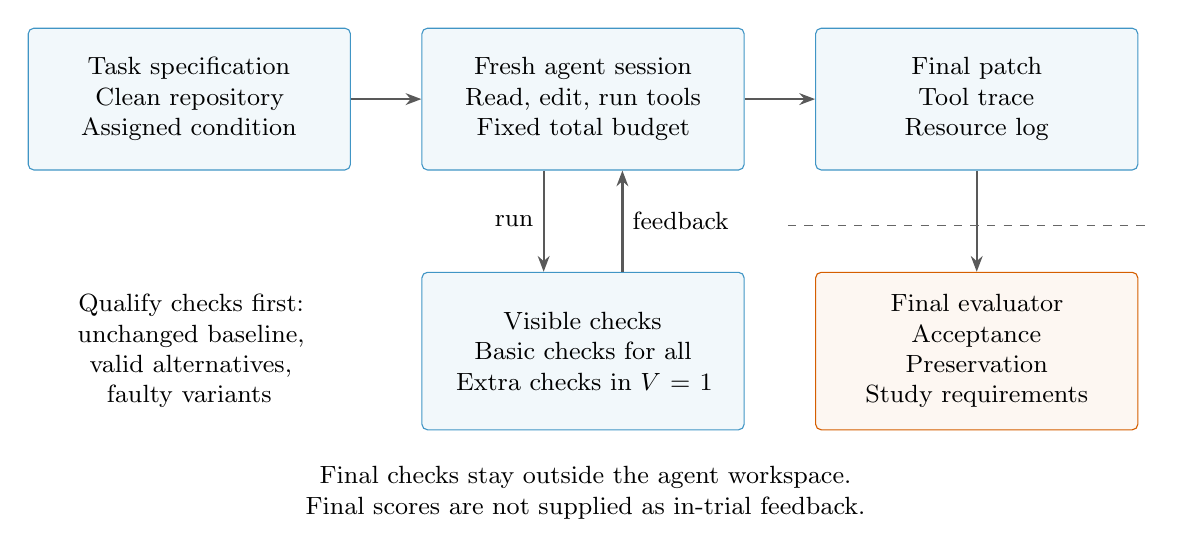
\begin{tikzpicture}
\node[box,text width=3.6cm,minimum height=18mm] (input) at (0,0) {Task specification\\Clean repository\\Assigned condition};
\node[box,text width=3.6cm,minimum height=18mm] (agent) at (5,0) {Fresh agent session\\Read, edit, run tools\\Fixed total budget};
\node[box,text width=3.6cm,minimum height=18mm] (patch) at (10,0) {Final patch\\Tool trace\\Resource log};
\node[box,text width=3.6cm,minimum height=20mm] (visible) at (5,-3.2) {Visible checks\\Basic checks for all\\Extra checks in $V=1$};
\node[box,text width=3.6cm,minimum height=20mm,draw=studyorange,fill=studyorange!5] (hidden) at (10,-3.2) {Final evaluator\\Acceptance\\Preservation\\Study requirements};
\node[note,text width=3.6cm] at (0,-3.2) {Qualify checks first:\\unchanged baseline,\\valid alternatives,\\faulty variants};
\draw[arrow] (input)--(agent);
\draw[arrow] (agent)--(patch);
\draw[arrow] ([xshift=-5mm]agent.south)--node[left,font=\small]{run} ([xshift=-5mm]visible.north);
\draw[arrow] ([xshift=5mm]visible.north)--node[right,font=\small]{feedback} ([xshift=5mm]agent.south);
\draw[arrow] (patch)--(hidden);
\draw[dashed,draw=black!60] (7.6,-1.6)--(12.2,-1.6);
\node[note,text width=13cm] at (5,-5) {Final checks stay outside the agent workspace.\\Final scores are not supplied as in-trial feedback.};
\end{tikzpicture}
\caption{Agents can run the checks supplied in their condition. The same final evaluator scores every saved patch for a given kit and task.}
\label{fig:evaluation}
\end{figure}


\subsection{What counts as success}\label{sec:outcomes}
Acceptance ($A$) passes when all checks for the requested behavior pass. Preservation ($P$) passes when all checks for specified existing behavior pass. For display names, the evaluator checks normalization on save and verifies that opening settings still shows an unedited legacy name as stored.

The common study requirements ($G$) pass when the patch passes the basic checks, keeps the supplied dependencies and existing public routes, and retains the assigned paths of the modules that define the layout comparison. The protocol will list the protected paths and routes before collection. Agents can edit modules in place and add files within the assigned layout. We will record compliance separately from the two behavioral scores.

Joint success is the primary binary outcome. An assessable session succeeds if $A$, $P$, and $G$ all pass. A known failure on any component establishes joint failure. If the agent produces no evaluable patch within budget or its changes block build or execution, we record joint failure and leave any unscorable components unassessed.

If an infrastructure failure blocks scoring, we will re-evaluate the saved patch when possible using the same evaluator. The result belongs to the original session. If scoring remains blocked and the joint outcome is undetermined, we record it as missing. Each scheduled session remains in the analysis dataset.

To interpret failures, we will use evaluator outputs and available traces to describe omitted behavior, incorrect changes, and check use. Navigation summaries will count searches, distinct source files read, and repeated reads after mapping moved files to the same modules~\cite{trivedi2026cleanliness}. We will record missing trace fields and distinguish uncertain author-coded interpretations from observed events.

\subsection{Validation of the scoring checks}
Before collection, we will map each task requirement to a check. In each kit and layout, the baseline must pass all preservation checks and fail at least one acceptance check. The reference patch must pass both sets. We will repeat evaluations on reset application state to check consistency. Because coverage and mutation scores provide indirect evidence of test effectiveness~\cite{inozemtseva2014coverage,just2014mutants,zhao2026coverage}, we will also test which valid alternatives and deliberate faults the evaluator accepts or detects~\cite{barr2015oracle,liu2023evalplus}.

Browser checks will exercise the form, keyboard, and session requirements. Database queries will verify the stored display name. For the visibility task, the completed matrix covers initial sign-in masking and toggle behavior. Before collection, we will also check sign-up masking and compare autocomplete against the corresponding baseline. The final evaluator will use its own copy of the checks.

\subsection{Comparing the four conditions}\label{sec:contrasts}
For RQ1, we will report joint success, acceptance, and preservation as passes over assessable sessions by kit, task, and condition, with missing counts.

For RQ2, we will subtract the original-layout joint success rate from the reorganized-layout rate at each check level and average the two differences. For RQ3, we will subtract the basic-only rate from the rate with extra checks within each layout and average those differences. Tasks receive equal weight within a kit, and the pooled estimates weight the two kits equally. We use assigned access regardless of whether the agent runs the extra checks. The interaction, the difference in the check-access effect between layouts, is descriptive.

We will report the contrasts in percentage points. With missing joint outcomes, we will bound each contrast over the scheduled sessions by filling unknown outcomes in the direction that minimizes or maximizes it. For complete data, simultaneous conservative 95\% Hoeffding intervals for the two pooled effects have a half-width of 42.7 percentage points under independent bounded session outcomes. Shared execution conditions can violate that assumption. We will report kit-specific contrasts descriptively and repeat the pooled comparison after omitting each matched task pair. Repeated runs help characterize stochastic variation~\cite{arcuri2014statistics}, but this design may leave even practically relevant differences unresolved.

Any secondary exact randomization tests will be specified in the protocol before collection, including their within-block comparisons, treatment of missing outcomes, and Holm adjustment across the two sharp nulls~\cite{holm1979multiple}.

As a secondary audit, we will apply the supplied and withheld preservation suites to the same saved patches in all conditions. We will cross-tabulate paired outcomes and report how many pairs could not be assessed. A preservation escape occurs when the supplied suite passes and the withheld suite fails. For each task, we will illustrate the first assessable joint failure in allocation order, or the first assessable patch if none fail.

We plan to release task specifications, evaluator code, configuration, analysis scripts, and results after reviewing the package for sensitive material. The scope of source redistribution depends on licenses and permissions. Test fixtures use synthetic records, and released traces and archives will exclude credentials.

\section{Preliminary evaluator qualification}\label{sec:results}\label{sec:account-qualification}
We completed \textbf{72 evaluator runs} to check scoring on baselines, reference patches, and deliberately faulty patches. For each kit, task, and layout, we evaluated all three versions twice with fresh data. The total was $2\,\text{kits}\times3\,\text{tasks}\times2\,\text{layouts}\times3\,\text{versions}\times2\,\text{rounds}=72$ runs. Chromium exercised the forms and controls, and database queries verified the stored display names.

Table~\ref{tab:qualification} summarizes the verdicts for the behaviors exercised in this matrix. All 24 reference cases passed the acceptance and preservation checks exercised. All 24 deliberately faulty cases passed the basic browser checks, while the task-specific checks detected every deliberate regression. The faults affected the display of unedited legacy names, session termination after sign-out, and initial sign-in password masking. Figure~\ref{fig:signout-example} shows how the session check distinguishes the two prepared sign-out patches. We also ran TypeScript checks on both layouts.

\begin{table}[htbp]
\centering
\small
\caption{Preliminary verdicts on baselines, reference patches, and deliberate regressions}
\label{tab:qualification}
\begin{tabularx}{\linewidth}{@{}lYYY@{}}
\toprule
Starter kit & Baseline failed acceptance and passed preservation & Reference passed both & Regression detected\\
\midrule
Next.js SaaS Starter & 12/12 & 12/12 & 12/12\\
Makerkit Lite & 12/12 & 12/12 & 12/12\\
\bottomrule
\end{tabularx}
\end{table}

\begin{figure}[htbp]
\centering
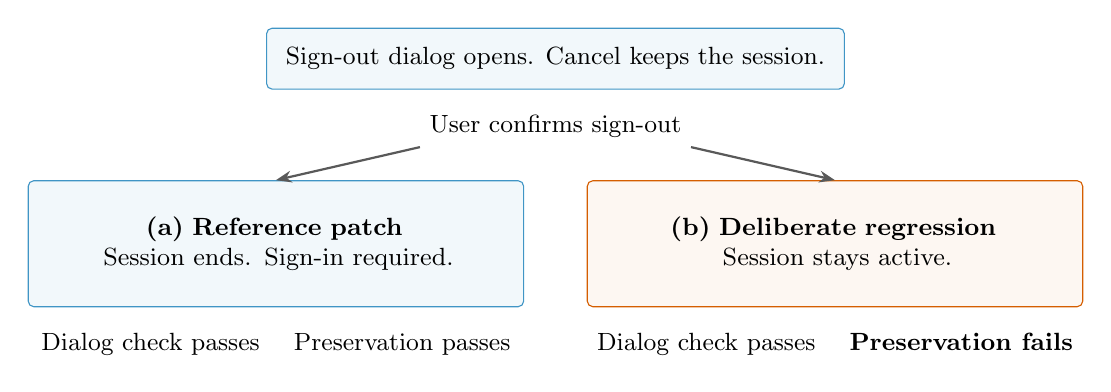
\begin{tikzpicture}
\node[box] (confirm) at (0,0) {Sign-out dialog opens. Cancel keeps the session.};
\node[note,below=2mm of confirm] (action) {User confirms sign-out};
\node[box,text width=5.8cm,minimum height=16mm] (reference) at (-3.55,-2.35)
  {\textbf{(a) Reference patch}\\Session ends. Sign-in required.};
\node[box,text width=5.8cm,minimum height=16mm,draw=studyorange,fill=studyorange!5] (regression) at (3.55,-2.35)
  {\textbf{(b) Deliberate regression}\\Session stays active.};
\draw[arrow] (action.south west) -- (reference.north);
\draw[arrow] (action.south east) -- (regression.north);
\node[note,below=2mm of reference] {Dialog check passes \quad Preservation passes};
\node[note,below=2mm of regression] {Dialog check passes \quad \textbf{Preservation fails}};
\end{tikzpicture}
\caption{Both prepared patches display the sign-out dialog. The preservation check detects the patch that leaves the session active after confirmation.}
\label{fig:signout-example}
\end{figure}


In one rehearsal per kit, we reapplied a prepared bundle to the reorganized layout and scored it on fresh data. Both bundles passed the task checks and included an alternative display-name implementation. The audit of 24 candidate packages confirmed that the paired $V=0$ and $V=1$ packages used identical application code, lockfiles, and task specifications.

\section{Discussion and threats to validity}
\subsection{Intervention interpretation}
The layout estimate covers the combined changes in file placement and imports. The package estimate includes the examples and execution feedback the checks supply, as well as the time they take to run. Traces can show whether edits follow check execution. Isolating the effect of feedback would require a control with equivalent information and different execution access.

\subsection{Evaluator scope and author involvement}
The author selects the tasks, designs the evaluator, and codes failures. These choices may favor familiar implementations, and independent review is currently unavailable. The supplied and withheld suites may share observations such as initial password masking, so agreement between them may partly reflect overlap. Qualification covers local Chromium and database behavior. Some Makerkit Lite settings pages showed hydration warnings during those runs.

\subsection{Task coverage, uncertainty, and transfer}
The three tasks qualify because the extra checks detect a prepared regression missed by the basic browser checks in both layouts. This selection favors tasks for which the package could be useful. The estimates apply to these tasks, kits, and the chosen agent configuration and budget. Shared infrastructure, caching, and model drift may affect session outcomes or timing.

\begin{samepage}
\section{Work plan}
\begin{enumerate}
\item Complete the task-to-layout audit and the requirement-to-check map. Rehearse patch capture and scoring, then fix the agent configuration, allocation, scoring rules, and analysis plan in the protocol.
\item Run the 48 scheduled sessions in the randomized order and retain the patch and run status for each session.
\item Score the patches, estimate the two effects, and analyze disagreements between the supplied and withheld preservation checks.
\end{enumerate}

Supervisor feedback is requested on whether the layout changes reach enough task-relevant code and whether the 48-session design fits the exploratory aim. If the layout audit shows insufficient changes to task-relevant paths, a two-kit comparison of check access remains a fallback for discussion.
\end{samepage}

\FloatBarrier
\bibliographystyle{abbrvnat}
\begingroup
\small
\setlength{\bibsep}{0pt}
\raggedright
\bibliography{references}
\endgroup
\end{document}
